\chapter{Lecture 9 - Multidimensional data}

\begin{figure}[htbp]
    \centering
    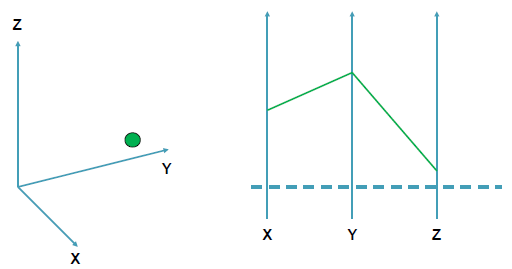
\includegraphics[width=0.3\linewidth]{imgs/lecture9/9.1 parallel coordinates.png}
    \caption{Parallel coordinates and cartesian coordinates}
    \label{fig:9.1}
\end{figure}
Parallel coordinates can be used to visualize multivariate data as an extension of Cartesian coordinates. Note that the order of the axes plays a fundamental role in its readability. 

Together with parallel coordinates, scatterplot matrices can be used to represent multidimensional data (among other visualization tools). However, a different approach exists, which is to \textit{reduce the dimensionality} of the data. This is a widely used strategy to map the dimensionality of the dataset from a higher N-dimension to 2 or 3 dimensions for a better understanding. Note that dimensionality reduction is a mapping, not a geometric transformation. It has different techniques, each with different properties.

\section{PCA - Principal Component Analysis}
PCA is a linear, non-parametric multidimensional reduction technique. The core idea is to find a basis formed by the directions that maximize the variance of the data, so that it can express the data in a new basis that best expresses our dataset. \par
Mathematically, if \(X\) is our original dataset and \(P\) is the transformation matrix, the new data \(Y\) is obtained as \(Y = XP\). In this transformation, each row of \(P(p_1, \dots ,p_m )\) represents a new direction (principal component), and \(Y\) represents the projection of the original data onto these directions

\begin{equation}
    \label{eq:9.1}
    PX = 
    \begin{bmatrix}
        \mathbf{p}_1 \\
        \vdots \\
        \mathbf{p}_m
    \end{bmatrix}
    [\mathbf{x}_1 \ \ldots \ \mathbf{x}_n]
\end{equation}

\subsubsection{Covariance Matrix}
The role of the covariance matrix is to find the best directions. PCA looks at the covariance Matrix (\(C_X\)) of the original data such that \(C_X = 1/(n-1)XX^T\), where the diagonal terms represent the variance of every single variable, while off-diagonal terms represent the covariance (redundancy) between different variables.\par
The goal is to find a matrix \(P\) such that the covariance matrix of the transformed data (\(C_Y\) is diagonalized, in other words, a matrix \(P\) that maximizes the variance and minimizes the redundancy. 
\begin{itemize}[noitemsep]
    \item Maximize variance implies that high values on the diagonal mean the dynamics of the variables are captured effectively.
    \item Minimize redundancy implies that the low off-diagonal values mean variables are no longer redundant.
\end{itemize}

\subsubsection{Solving PCA}
\begin{theorem}
    A symmetric matrix \(A\) can be diagonalized by a matrix formed by its eigenvectors as \(A = EDE^T\), where the columns of \(E\) are the eigenvectors of \(A\).
\end{theorem}

The solution relies on Theorem 9.1. The steps to compute PCA are:
\begin{enumerate}[noitemsep]
    \item Organize data as a \(m \times n\) matrix
    \item Subtract the mean from each row
    \item Calculate the eigenvalues and eigenvectors of \(XX^T\)
    \item The eigenvectors organized by their corresponding eigenvalues from the matrix \(P\)
\end{enumerate}

Remember that \(Y=PX\), we define the covariance matrix of the new data \(C_Y = 1/(n-1)YY^T\)
\begin{enumerate}[noitemsep]
    \item substitute \(Y\) with \(PX\): \(= 1/(n-1)(PX)(PX)^T\)
    \item resolve the equation: \(= 1/(n-1)PXX^TP^T\)
    \item apply the theorem 9.1: \(= 1/(n-1)P(XX^T)P^T\)
    \item as the result of Theorem 9.1, we obtain that \(C_Y = 1/(n-1)PAP^T\), where \(P\) is transformation matrix and \(A\) is the symmetric matrix
\end{enumerate}

\subsubsection{Reducing dimensionality and reconstruction error}
Reduction occurs when we choose only the first \(k\) principal components (\(k < m\)). By projecting the data onto these \(k\) directions, we get a lower-dimensional representation that is the best approximation of the original data. \par
PCA minimizes the reconstruction error \(e\), defined as the sum of squared differences between the original points (\(y_i\)) and the projected points (\(\tilde{y_i}\)):

\begin{equation}
    \label{eq:9.2}
    e = \sum_i^k(\tilde{y_i} - y_i)^2
\end{equation}

In fig. \ref{fig:9.2} shows a visual example of a ball attached to a spring moving along a single axis (the x-axis). If three different cameras record this movement, the raw data has 6 dimensions (x, y, coordinates for each of the 3 cameras). Because the ball only moves in 1D, most of these 6 dimensions are redundant or contain noise, but applying PCA allows the system to identify the single primary direction of motion, effectively reducing 6 noisy dimensions back to the 1 meaningful dimension that captures the most variance.
\begin{figure}[htbp]
    \centering
    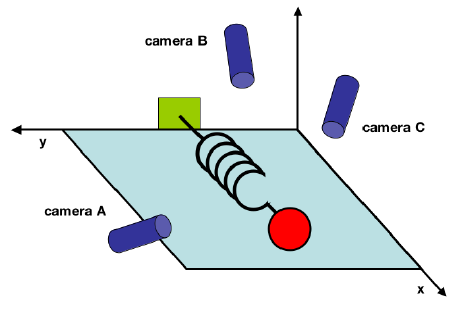
\includegraphics[width=0.5\linewidth]{imgs/lecture9/9.2 PCA example.png}
    \caption{visual example of PCA dimensionality reduction}
    \label{fig:9.2}
\end{figure}

\subsubsection{Limitations}
\begin{itemize}[noitemsep]
    \item Non-parametric: while a strength, it can be a weakness because it does not incorporate prior knowledge
    \item distribution: it fails for data that is not Gaussian-distributed
    \item linearity: it is a linear technique; for non-linear structures, extensions like kernel PCA or other methods are needed
    \item independence: PCA does not guarantee statistical independence
\end{itemize}

\section{MDS - Multi-Dimensional Scaling}
MDS is a classic technique for dimensionality reduction. The primary rationale behind MDS is to find a lower-dimensional representation of data that preserves the pairwise distances between points as accurately as possible.
\begin{itemize}
    \item The mapping: it seeks a linear mapping (\(y_i = Mx_i\)) that minimizes a cost function (\(\phi(Y)\)) representing the differences between the Euclidean distance of points in the high-dimensional space (\(d_{ij}^2\)) and their distance in the low-dimensional space (\(||y_i - y_j||^2\))
    \begin{equation}
        \phi(Y) = \sum_{i, j} d^2_{ij} - || y_i - y_j||^2
    \end{equation}
    \item relationship to PCA: minimizing the distance mismatch (\(\phi(Y)\)) is mathematically equivalent to maximizing the variance of the points in the new space, which is the exact goal of PCA.
\end{itemize}

\subsubsection{MDS vs PCA}
While the two techniques share similar goals and both better preserve large pairwise distances, they differ significantly in their computational scaling:
\begin{itemize}
    \item PCA scales based on the dimensions of the data (the size of the covariance matrix is proportional to the number of variables)
    \item MDS scales based on the number of data points. This makes MDS a distinct choice depending on whether a dataset has many variables or many individual samples.
\end{itemize}

\subsubsection{Sammon mapping variant}
It is a specific adaptation of MDS that allows for retaining the local structure of the data better than classical MDS, where retention of high distances is privileged, and not of local structure. Sammon mapping addresses this by weighting the contribution of each pair of points.

\section{LLE - Locally Linear Embedding}
LLE is a dimension reduction technique designed to discover non-linear structures in high-dimensional data by exploiting local linear approximations. While PCA is a linear technique that looks at global variance. LLE operates on the intuition that even if a dataset is globally non-linear, it can be approximated as locally linear.

\subsubsection{Core intuition}
The fundamental assumption of LLE is that the high-dimensional data lies on a "well-sampled" manifold. Because the manifold is well-sampled, any given data point and its immediate neighbors can be treated as a small, locally linear patch. Each point in this patch can be represented as a weighted sum of its neighbors.

\subsubsection{The LLE algorithm}
LLE follows a three-step mathematical process to map high-dimensional points into a lower-dimensional space:
\begin{enumerate}[noitemsep]
    \item \textbf{identify neighbors}: for every data point \(X_i\) in the high-dimensional space, the algorithm finds its K-nearest neighbors or all points within a specific ball radius.
    \item \textbf{compute reconstruction weights}: the algorithm calculates the weights \(W_{ij}\) that best reconstruct each point \(X_i\) from its neighbors by minimizing the error function: 
    \begin{equation}
        \label{eq:9.3}
        \epsilon(W) = \sum_i | X_i - \sum_j W_{ij} X_j|^2
    \end{equation}
    In this step, the weights capture the local geometric properties of the data
    \item \textbf{map to low-dimensional space}: finally, the algorithm finds new vectors \(Y_i\) in a lower-dimensional space (2D or 3D) that respect those same weights. It does this by minimizing a new cost function while keeping the weights \(W_{ij}\) fixed:
    \begin{equation}
        \label{eq:9.4}
        \Phi(Y) = \sum_i |Y_i - \sum_j W_{ij}Y_j|^2
    \end{equation}
    This ensures that the local neighborhood relationships from the original high-dimensional space are preserved in the new, reduced space.
\end{enumerate}

\section{Isomap}
The Isomap is a dimensionality reduction technique based in the core principle of preserving the geodesic distance between data points. It is designed to understand the intrinsic geometry of a curved space (a manifold).\par
In a high-dimensional space where data lies on a curved surface, the straight-line Euclidean distance between two points can be misleading because it "cuts through" the empty space of the manifold.
\begin{definition}[Geodesic Distance]
    Geodesic distance is the shortest path between two points measured along the surface of the curved space.
\end{definition}
An isomap aims to "unroll" this curved manifold into a flat representation while keeping the distances along the surface consistent.

\subsubsection{Procedure}
The Isomap algorithm can be seen as a three-step mathematical procedure:
\begin{enumerate}[noitemsep]
    \item \textbf{construct neighborhood graph (\(G\))}: define a graph over all data points by connecting all points (i, j) if and only if point \(i\) is one of the K-nearest neighbors of point \(j\)
    \item \textbf{compute the shortest path}: using Floyd's algorithm (or a similar shortest-path algorithm) to calculate the shortest path between all pairs of points in the graph \(G\). This results in an approximation of the global geodesic distances between all points in the dataset.
    \item \textbf{construct the d-dimensional embedding}: use the matrix of approximated geodesic distances to find a lower-dimensional representation.
\end{enumerate}

\subsubsection{Applications}
Isomap is particularly effective for datasets where the "meaningful" dimensions are non-linear:
\begin{itemize}[noitemsep]
    \item Face poses: when applied to a dataset of faces, Isomap can successfully map images onto axes representing "up-down pose" and "left-right pose", capturing the natural rotation of a head
    \item Handwriting: Isomap can be used to visualize how different digits vary based on their "top arch" or "bottom loop" articulation
\end{itemize}

\section{Autoencoder}
An autoencoder is a specialized type of neural network used to perform dimensionality reduction. These networks offer a powerful way to map complex data into simpler forms. A multi-layer autoencoder consists of two primary components that work together to process data:
\begin{itemize}[noitemsep]
    \item The \textbf{encoder} that takes the high-dimensional \textbf{input data X}, and passes it through several layers of neurons. Each layer uses a set of weights to progressively compress the information. 
    \item At the center of the network is a \textbf{"bottleneck" layer}. This layer holds the compressed, \textbf{low-dimensional representation (Y)} of the input data, effectively capturing its most essential features
    \item The \textbf{decoder} performs the reverse operation of the encoder by using a mirrored set of transposed weights to attempt to reconstruct the original data from the compressed representation. Thus, obtaining the final \textbf{output data X'}
\end{itemize}

\begin{figure}[htbp]
    \centering
    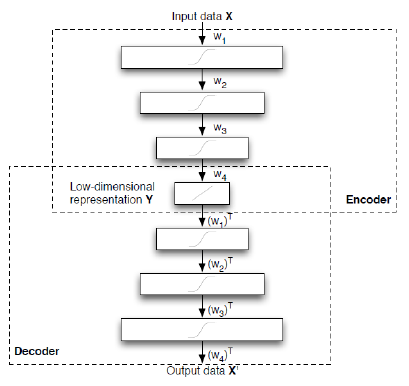
\includegraphics[width=0.4\linewidth]{imgs/lecture9/9.3 autoencoder.png}
    \caption{Multi-layer autoencoder}
    \label{fig:9.3}
\end{figure}

The network is trained to ensure that the output data X' is as close to the input data X as possible. Because the data must pass through the low-dimensional bottleneck Y, the autoencoder is forced to learn a highly efficient way to represent the data. \par
To make it work for dimensionality reduction, once the network is trained, the decoder part can be discarded, and the encoder can be used as a tool to transform high-dimensional datasets into a 2D or 3D representation for visualization and analysis, similar to the goals of PCA or Isomap.

\section{t-SNE}
t-SNE stands for t-Distributed Stochastic Neighbor Embedding, a state-of-art dimensionality reduction technique to a common problem: the inability of most techniques to retain both local and global structure of data in a single 2D or 3D map.

\subsection{SNE}
Before introducing t-SNE, it is important to understand its predecessor. SNE models the relationships between data points using conditional probability rather than fixed distances. 
\begin{itemize}
    \item High-dimensional similarity (\(p_{j|i}\)): in the original high-dimensional space, the similarity of point \(x_j\) to point \(x_i\) is the probability that \(x_i\) would pick \(x_j\) as its neighbor. This is calculated using a Gaussian distribution centered at \(x_i\)
    \item Low-dimensional similarity (\(q_{j|i}\)): an analogous probability is calculated for the points in the lower-dimensional space
\end{itemize}
The objective is to ensure that the low-dimensional map Q reflects the high-dimensional neighborhood structure P as closely as possible, i.e., minimizes the mismatch between \(p_{j|i}\) and \(q_{j|i}\), this can be achieved using the KL divergence.

\subsection{Kullback-Leibler (KL) Divergence}
To quantify how much the low-dimensional map differs from the original data, SNE uses KL Divergence, also known as relative entropy.
\begin{itemize}
    \item Coding theory view: it represents the expected number of extra bits required to code samples from distribution \(P\) if the code is optimized for distribution \(Q\).
    \item Bayesian view: it measures the information gained when one revises beliefs from a prior distribution Q to a posterior distribution P.
    \item Mathematical property: a critical detail noted in the sources is that KL divergence is not symmetric, meaning \(KL(P||Q) \neq KL (Q||P)\).
\end{itemize}

\subsection{Into t-SNE}
Standard SNE has two major flaws: its cost function is difficult to optimize, and it suffers from the "crowding problem", where points in the low-dimensional map tend to collapse together into a cluttered center. t-SNE solves these through two specific innovations:
\begin{itemize}[noitemsep]
    \item \textbf{Symmetry}: t-SNE makes the SNE cost function symmetric, which simplifies the optimization process \(KL(P||Q) = KL (Q||P)\)
    \item \textbf{Student-t distribution}: instead of the Gaussian distribution, t-SNE uses the Student-t distribution with one degree of freedom to evaluate similarities in the low-dimensional space. The "heavy tails" of the Student-t distribution allow points that are far apart in the high-dimensional space to be modeled as even farther in the low-dimensional space, which effectively alleviates the crowding problem.
\end{itemize}